\chapter{Elicitação de Requisitos e Análise}
\label{cap:05}

Este capítulo apresenta o processo de elicitação e análise dos requisitos do
sistema especialista educacional para validação de compatibilidade de
\textit{hardware}. Inicialmente, são descritos os requisitos do usuário e do
sistema, classificados em funcionais e não funcionais. Em seguida, são
apresentados os artefatos de análise: casos de uso, modelo de domínio e
diagrama de classes de análise, que descrevem a estrutura e o comportamento
esperados da aplicação.

\section{Requisitos do Usuário}

Os requisitos do usuário expressam, em linguagem natural, as necessidades que
motivam o desenvolvimento do sistema do ponto de vista de quem o utiliza. O
usuário-alvo deste trabalho é o consumidor leigo que pretende montar um
computador \textit{desktop} e necessita verificar a compatibilidade entre os
componentes selecionados.

Nesse contexto, o sistema deve permitir que o usuário selecione componentes de
\textit{hardware} de forma guiada e, a cada seleção, seja informado de imediato
sobre quais componentes se tornam incompatíveis e, sobretudo, sobre a razão
técnica de cada incompatibilidade. Diferentemente das plataformas comerciais
existentes, que apenas sinalizam o conflito, o sistema proposto deve transformar
cada bloqueio em uma oportunidade de aprendizagem, comunicando ao usuário a
regra física ou lógica violada em linguagem acessível.

\section{Requisitos do Sistema}

Os requisitos do sistema traduzem as necessidades do usuário em especificações
detalhadas que orientam o projeto e a implementação. Segundo
\textcite{sommerville2011}, os requisitos de sistema são descrições mais
detalhadas das funções, dos serviços e das restrições operacionais do
\textit{software}, servindo de contrato entre o que se espera e o que será
construído. Assim, esta seção apresenta os requisitos identificados neste
trabalho, organizados em funcionais e não funcionais.

\subsection{Requisitos Funcionais}

De acordo com \textcite{sommerville2011}, os requisitos funcionais descrevem o
que o sistema deve fazer, isto é, os serviços que ele deve fornecer, como deve
reagir a determinadas entradas e como deve se comportar em situações
específicas.

Os atores que interagem com o sistema são: usuário e sistema. Os requisitos
funcionais identificados estão apresentados nos Quadros~\ref{quad:rf01}
a~\ref{quad:rf19}.

Os requisitos estão classificados quanto à prioridade
(\textit{Essencial}, \textit{Importante} ou \textit{Desejável}) e
quanto à operação (\textit{Entrada}, \textit{Processamento} ou \textit{Saída}).

% ----------------------------------------------------------
%  RF-01
% ----------------------------------------------------------
\FloatBarrier
\begin{quadro}[htb]
  \caption{RF-01 -- Listar componentes por categoria}
  \label{quad:rf01}
  \begin{tabular}{|p{3.2cm}|p{11.8cm}|}
    \hline
    \textbf{Código}     & RF-01                                                                                     \\ \hline
    \textbf{Grupo}      & Catálogo de Componentes                                                                   \\ \hline
    \textbf{Descrição}  &
    \textbf{Ação:} Listar.
    \textbf{Objeto:} Componentes de \textit{hardware} agrupados por categoria.
    \textbf{Atributos:} categoria (variável do CSP), nome do modelo, características associadas à categoria e seus respectivos valores.
    \textbf{Exemplos:} Usuário acessa o sistema e visualiza a lista de componentes da primeira categoria cadastrada (ex.: CPU); usuário avança e visualiza a lista de componentes da categoria seguinte.
    \textbf{Restrições:}
    \begin{enumerate}[nosep,leftmargin=1.2em,topsep=2pt,partopsep=0pt,parsep=0pt,itemsep=1pt]
      \item O catálogo deve ser exibido separado por categoria.
      \item As categorias exibidas devem ser obtidas dinamicamente da base de conhecimento, não fixadas no código.
      \item Cada componente deve exibir as características associadas à sua categoria, relevantes à compatibilidade.
    \end{enumerate} \\ \hline
    \textbf{Prioridade} & Essencial                                                                                 \\ \hline
    \textbf{Operação}   & Saída                                                                                     \\ \hline
    \textbf{Ator}       & Usuário                                                                                   \\ \hline
  \end{tabular}
  \fonte{Elaborada pelo autor}
\end{quadro}

% ----------------------------------------------------------
%  RF-02
% ----------------------------------------------------------
\FloatBarrier
\begin{quadro}[htb]
  \caption{RF-02 -- Navegar pela interface \textit{wizard}}
  \label{quad:rf02}
  \begin{tabular}{|p{3.2cm}|p{11.8cm}|}
    \hline
    \textbf{Código}     & RF-02                                                                                       \\ \hline
    \textbf{Grupo}      & Catálogo de Componentes                                                                     \\ \hline
    \textbf{Descrição}  &
    \textbf{Ação:} Navegar.
    \textbf{Objeto:} Interface \textit{wizard} de configuração passo a passo.
    \textbf{Atributos:} etapa atual, categoria de componente em seleção.
    \textbf{Exemplos:} Usuário conclui a seleção da CPU e avança para a etapa de Placa-mãe; usuário retorna à etapa anterior para revisar a seleção.
    \textbf{Restrições:}
    \begin{enumerate}[nosep,leftmargin=1.2em,topsep=2pt,partopsep=0pt,parsep=0pt,itemsep=1pt]
      \item A interface deve guiar o usuário sequencialmente por cada categoria de \textit{hardware}.
      \item A ordem das etapas deve ser determinada pela ordenação das categorias cadastradas na base de conhecimento.
      \item O usuário deve poder avançar e retroceder entre etapas.
    \end{enumerate} \\ \hline
    \textbf{Prioridade} & Essencial                                                                                   \\ \hline
    \textbf{Operação}   & Entrada                                                                                     \\ \hline
    \textbf{Ator}       & Usuário                                                                                     \\ \hline
  \end{tabular}
  \fonte{Elaborada pelo autor}
\end{quadro}

% ----------------------------------------------------------
%  RF-03
% ----------------------------------------------------------
\FloatBarrier
\begin{quadro}[htb]
  \caption{RF-03 -- Exibir componentes incompatíveis com sinalização visual}
  \label{quad:rf03}
  \begin{tabular}{|p{3.2cm}|p{11.8cm}|}
    \hline
    \textbf{Código}     & RF-03                                                                \\ \hline
    \textbf{Grupo}      & Catálogo de Componentes                                              \\ \hline
    \textbf{Descrição}  &
    \textbf{Ação:} Exibir com sinalização visual de bloqueio.
    \textbf{Objeto:} Componentes incompatíveis com a seleção atual.
    \textbf{Atributos:} status de compatibilidade, indicador visual de bloqueio.
    \textbf{Exemplos:} Após seleção de CPU com soquete AM5, todas as placas-mãe com soquete AM4 permanecem visíveis na lista, porém exibidas com indicador de bloqueio.
    \textbf{Restrições:}
    \begin{enumerate}[nosep,leftmargin=1.2em,topsep=2pt,partopsep=0pt,parsep=0pt,itemsep=1pt]
      \item Componentes incompatíveis \textbf{não} devem ser ocultados da listagem.
      \item Devem ser mantidos visíveis com indicador visual de bloqueio.
      \item O usuário deve poder visualizar o motivo do bloqueio ao interagir com o componente.
    \end{enumerate} \\ \hline
    \textbf{Prioridade} & Essencial                                                            \\ \hline
    \textbf{Operação}   & Saída                                                                \\ \hline
    \textbf{Ator}       & Usuário                                                              \\ \hline
  \end{tabular}
  \fonte{Elaborada pelo autor}
\end{quadro}

% ----------------------------------------------------------
%  RF-04
% ----------------------------------------------------------
\FloatBarrier
\begin{quadro}[htb]
  \caption{RF-04 -- Exibir características técnicas dos componentes}
  \label{quad:rf04}
  \begin{tabular}{|p{3.2cm}|p{11.8cm}|}
    \hline
    \textbf{Código}     & RF-04                                                                                                  \\ \hline
    \textbf{Grupo}      & Catálogo de Componentes                                                                                \\ \hline
    \textbf{Descrição}  &
    \textbf{Ação:} Exibir.
    \textbf{Objeto:} Características técnicas do componente, derivadas da base de conhecimento.
    \textbf{Atributos:} pares característica--valor associados à categoria do componente -- variáveis conforme a categoria.
    \textbf{Exemplos:} \{Ryzen 5 7600: soquete = AM5, TDP = 65\,W\}; \{Kingston DDR5-5600: padrão = DDR5, capacidade = 16\,GB\}.
    \textbf{Restrições:}
    \begin{enumerate}[nosep,leftmargin=1.2em,topsep=2pt,partopsep=0pt,parsep=0pt,itemsep=1pt]
      \item As características devem ser exibidas para cada componente do catálogo.
      \item As características exibidas devem ser determinadas pela categoria do componente, não codificadas por tipo no sistema.
      \item A inclusão de uma nova característica não deve exigir alteração de código.
    \end{enumerate} \\ \hline
    \textbf{Prioridade} & Importante                                                                                             \\ \hline
    \textbf{Operação}   & Saída                                                                                                  \\ \hline
    \textbf{Ator}       & Usuário                                                                                                \\ \hline
  \end{tabular}
  \fonte{Elaborada pelo autor}
\end{quadro}

% ----------------------------------------------------------
%  RF-05
% ----------------------------------------------------------
\FloatBarrier
\begin{quadro}[htb]
  \caption{RF-05 -- Executar propagação de restrições via algoritmo AC-3}
  \label{quad:rf05}
  \begin{tabular}{|p{3.2cm}|p{11.8cm}|}
    \hline
    \textbf{Código}     & RF-05                                                                                                              \\ \hline
    \textbf{Grupo}      & Motor de Inferência (CSP/AC-3)                                                                                     \\ \hline
    \textbf{Descrição}  &
    \textbf{Ação:} Executar propagação de restrições.
    \textbf{Objeto:} Algoritmo AC-3 sobre o grafo de restrições do CSP, construído dinamicamente a partir da base de conhecimento.
    \textbf{Atributos:} estado atual das seleções do usuário, domínios das variáveis (categorias cadastradas), fila de arcos derivada das restrições persistidas.
    \textbf{Exemplos:} Usuário seleciona uma CPU com soquete AM5; o AC-3 é invocado e remove do domínio da categoria vizinha (Placa-mãe) todos os modelos cujo valor de característica viole a restrição cadastrada.
    \textbf{Restrições:}
    \begin{enumerate}[nosep,leftmargin=1.2em,topsep=2pt,partopsep=0pt,parsep=0pt,itemsep=1pt]
      \item O AC-3 deve ser invocado a cada seleção de componente realizada pelo usuário.
      \item O grafo de restrições deve ser montado em tempo de execução a partir das restrições cadastradas, sem regras codificadas no motor.
      \item O estado completo das seleções deve ser enviado à API REST a cada chamada (arquitetura \textit{stateless}).
      \item O resultado deve retornar os domínios atualizados em tempo real, sem atraso perceptível.
      \item A complexidade de pior caso deve ser $O(cd^{3})$, conforme definido por \textcite{Mackworth1977}.
    \end{enumerate} \\ \hline
    \textbf{Prioridade} & Essencial                                                                                                          \\ \hline
    \textbf{Operação}   & Processamento                                                                                                      \\ \hline
    \textbf{Ator}       & Sistema                                                                                                            \\ \hline
  \end{tabular}
  \fonte{Elaborada pelo autor}
\end{quadro}

% ----------------------------------------------------------
%  RF-06
% ----------------------------------------------------------
\FloatBarrier
\begin{quadro}[htb]
  \caption{RF-06 -- Validar compatibilidade de soquete CPU--Placa-mãe}
  \label{quad:rf06}
  \begin{tabular}{|p{3.2cm}|p{11.8cm}|}
    \hline
    \textbf{Código}     & RF-06                                                                             \\ \hline
    \textbf{Grupo}      & Motor de Inferência (CSP/AC-3)                                                    \\ \hline
    \textbf{Descrição}  &
    \textbf{Ação:} Validar.
    \textbf{Objeto:} Compatibilidade de soquete entre CPU e Placa-mãe (instância de restrição de igualdade do conjunto $C$).
    \textbf{Atributos:} soquete da CPU, soquete suportado pela placa-mãe.
    \textbf{Exemplos:} \{CPU: AM5, Placa-mãe: AM4\} $\rightarrow$ incompatível -- bloqueio acionado; \{CPU: AM5, Placa-mãe: AM5\} $\rightarrow$ compatível.
    \textbf{Restrições:}
    \begin{enumerate}[nosep,leftmargin=1.2em,topsep=2pt,partopsep=0pt,parsep=0pt,itemsep=1pt]
      \item A restrição é binária e absoluta -- não admite adaptação de \textit{software} ou configuração.
      \item O soquete da CPU deve ser idêntico ao soquete suportado pela placa-mãe.
      \item Incompatibilidade detectada deve bloquear o componente e acionar o módulo de explicação (RF-11).
    \end{enumerate} \\ \hline
    \textbf{Prioridade} & Essencial                                                                         \\ \hline
    \textbf{Operação}   & Processamento                                                                     \\ \hline
    \textbf{Ator}       & Sistema                                                                           \\ \hline
  \end{tabular}
  \fonte{Elaborada pelo autor}
\end{quadro}

% ----------------------------------------------------------
%  RF-07
% ----------------------------------------------------------
\FloatBarrier
\begin{quadro}[htb]
  \caption{RF-07 -- Validar padrão de memória RAM--Placa-mãe}
  \label{quad:rf07}
  \begin{tabular}{|p{3.2cm}|p{11.8cm}|}
    \hline
    \textbf{Código}     & RF-07                                                                             \\ \hline
    \textbf{Grupo}      & Motor de Inferência (CSP/AC-3)                                                    \\ \hline
    \textbf{Descrição}  &
    \textbf{Ação:} Validar.
    \textbf{Objeto:} Padrão de memória entre módulo RAM e Placa-mãe (instância de restrição de igualdade do conjunto $C$).
    \textbf{Atributos:} padrão DDR do módulo RAM (DDR4 ou DDR5), padrão DDR suportado pela placa-mãe.
    \textbf{Exemplos:} \{RAM: DDR4-3200, Placa-mãe: B650 (somente DDR5)\} $\rightarrow$ incompatível; \{RAM: DDR5-5600, Placa-mãe: B650\} $\rightarrow$ compatível.
    \textbf{Restrições:}
    \begin{enumerate}[nosep,leftmargin=1.2em,topsep=2pt,partopsep=0pt,parsep=0pt,itemsep=1pt]
      \item Os padrões DDR4 e DDR5 são física e eletricamente incompatíveis.
      \item O padrão do módulo deve corresponder exatamente ao suportado pela placa-mãe.
      \item A restrição é transitiva: depende da placa-mãe, que por sua vez depende da CPU selecionada.
      \item Incompatibilidade detectada deve bloquear o componente e acionar o módulo de explicação (RF-12).
    \end{enumerate} \\ \hline
    \textbf{Prioridade} & Essencial                                                                         \\ \hline
    \textbf{Operação}   & Processamento                                                                     \\ \hline
    \textbf{Ator}       & Sistema                                                                           \\ \hline
  \end{tabular}
  \fonte{Elaborada pelo autor}
\end{quadro}
% ----------------------------------------------------------
%  RF-08
% ----------------------------------------------------------
\FloatBarrier
\begin{quadro}[htb]
  \caption{RF-08 -- Validar capacidade energética da fonte (TDP)}
  \label{quad:rf08}
  \begin{tabular}{|p{3.2cm}|p{11.8cm}|}
    \hline
    \textbf{Código}     & RF-08                                                                                                                                                                                            \\ \hline
    \textbf{Grupo}      & Motor de Inferência (CSP/AC-3)                                                                                                                                                                   \\ \hline
    \textbf{Descrição}  &
    \textbf{Ação:} Validar.
    \textbf{Objeto:} Capacidade energética da fonte de alimentação em relação ao consumo de cada componente (instâncias de restrição quantitativa do conjunto $C$).
    \textbf{Atributos:} TDP da CPU (W), TDP da GPU (W), potência da fonte (W), margem de segurança recomendada (20--30\%).
    \textbf{Exemplos:} \{GPU TDP: 170\,W, Fonte: 250\,W\} $\rightarrow$ bloqueado (170\,W $\times$ 1,25 = 212,5\,W, porém a fonte deve suportar cada demanda com margem e a configuração completa a excede); \{GPU TDP: 170\,W, Fonte: 550\,W\} $\rightarrow$ válido.
    \textbf{Restrições:}
    \begin{enumerate}[nosep,leftmargin=1.2em,topsep=2pt,partopsep=0pt,parsep=0pt,itemsep=1pt]
      \item A fonte deve suprir a demanda energética de cada componente de maior consumo (CPU e GPU) individualmente, acrescida de margem de segurança de 20--30\%, preservando a natureza binária das restrições do grafo.
      \item A restrição é quantitativa (desigualdade), diferentemente das restrições binárias de soquete e memória.
      \item Fonte subdimensionada deve ser bloqueada e acionar o módulo de explicação com os valores calculados (RF-13).
      \item O consumo agregado da configuração é calculado e exibido ao usuário a título informativo, não constituindo restrição do CSP.
    \end{enumerate} \\ \hline
    \textbf{Prioridade} & Essencial                                                                                                                                                                                        \\ \hline
    \textbf{Operação}   & Processamento                                                                                                                                                                                    \\ \hline
    \textbf{Ator}       & Sistema                                                                                                                                                                                          \\ \hline
  \end{tabular}
  \fonte{Elaborada pelo autor}
\end{quadro}

% ----------------------------------------------------------
%  RF-09
% ----------------------------------------------------------
\FloatBarrier
\begin{quadro}[htb]
  \caption{RF-09 -- Propagar restrições incrementalmente a cada seleção}
  \label{quad:rf09}
  \begin{tabular}{|p{3.2cm}|p{11.8cm}|}
    \hline
    \textbf{Código}     & RF-09                                                                                      \\ \hline
    \textbf{Grupo}      & Motor de Inferência (CSP/AC-3)                                                             \\ \hline
    \textbf{Descrição}  &
    \textbf{Ação:} Propagar restrições e atualizar domínios.
    \textbf{Objeto:} Domínios das variáveis do CSP após cada interação do usuário.
    \textbf{Atributos:} variáveis afetadas, valores removidos dos domínios, arcos reinseridos na fila do AC-3.
    \textbf{Exemplos:} Remoção do valor AM5 do domínio de CPU provoca reinserção do arco (Placa-mãe, CPU) na fila para reverificação dos modelos de placa-mãe ainda disponíveis.
    \textbf{Restrições:}
    \begin{enumerate}[nosep,leftmargin=1.2em,topsep=2pt,partopsep=0pt,parsep=0pt,itemsep=1pt]
      \item A propagação deve ser incremental a cada interação, nunca por avaliação exaustiva (\textit{brute force}).
      \item O motor deve operar até o ponto de estabilidade -- quando nenhuma remoção adicional for possível.
    \end{enumerate} \\ \hline
    \textbf{Prioridade} & Essencial                                                                                  \\ \hline
    \textbf{Operação}   & Processamento                                                                              \\ \hline
    \textbf{Ator}       & Sistema                                                                                    \\ \hline
  \end{tabular}
  \fonte{Elaborada pelo autor}
\end{quadro}

% ----------------------------------------------------------
%  RF-10
% ----------------------------------------------------------
\FloatBarrier
\begin{quadro}[htb]
  \caption{RF-10 -- Exibir justificativa técnica para cada incompatibilidade}
  \label{quad:rf10}
  \begin{tabular}{|p{3.2cm}|p{11.8cm}|}
    \hline
    \textbf{Código}     & RF-10                                                               \\ \hline
    \textbf{Grupo}      & Explicações Educativas (\textit{Explanation Facility})              \\ \hline
    \textbf{Descrição}  &
    \textbf{Ação:} Exibir justificativa técnica em linguagem natural.
    \textbf{Objeto:} Incompatibilidade detectada pelo AC-3.
    \textbf{Atributos:} restrição violada, componentes envolvidos, princípio técnico subjacente.
    \textbf{Exemplos:} ``Este módulo de memória é incompatível: a placa-mãe compatível com o processador selecionado suporta exclusivamente DDR5, e este módulo utiliza o padrão DDR4.''
    \textbf{Restrições:}
    \begin{enumerate}[nosep,leftmargin=1.2em,topsep=2pt,partopsep=0pt,parsep=0pt,itemsep=1pt]
      \item Cada componente bloqueado deve ter uma justificativa exibida ao usuário.
      \item A justificativa deve identificar explicitamente qual restrição do CSP foi violada.
      \item A linguagem deve ser acessível ao usuário leigo.
      \item Nenhum bloqueio pode ocorrer de forma silenciosa (sem explicação ao usuário).
    \end{enumerate} \\ \hline
    \textbf{Prioridade} & Essencial                                                           \\ \hline
    \textbf{Operação}   & Saída                                                               \\ \hline
    \textbf{Ator}       & Sistema                                                             \\ \hline
  \end{tabular}
  \fonte{Elaborada pelo autor}
\end{quadro}

% ----------------------------------------------------------
%  RF-11
% ----------------------------------------------------------
\FloatBarrier
\begin{quadro}[htb]
  \caption{RF-11 -- Exibir alerta de incompatibilidade de soquete}
  \label{quad:rf11}
  \begin{tabular}{|p{3.2cm}|p{11.8cm}|}
    \hline
    \textbf{Código}     & RF-11                                                                     \\ \hline
    \textbf{Grupo}      & Explicações Educativas (\textit{Explanation Facility})                    \\ \hline
    \textbf{Descrição}  &
    \textbf{Ação:} Exibir alerta com explicação.
    \textbf{Objeto:} Incompatibilidade de soquete entre CPU e Placa-mãe.
    \textbf{Atributos:} soquete exigido pela CPU selecionada, soquete oferecido pela placa-mãe bloqueada.
    \textbf{Exemplos:} ``Esta placa-mãe utiliza soquete AM4, incompatível com o processador selecionado, que exige soquete AM5.''
    \textbf{Restrições:}
    \begin{enumerate}[nosep,leftmargin=1.2em,topsep=2pt,partopsep=0pt,parsep=0pt,itemsep=1pt]
      \item O alerta deve nomear explicitamente os dois soquetes envolvidos (ex.: AM4 e AM5).
      \item Deve ser exibido no momento em que o usuário tenta selecionar o componente incompatível.
    \end{enumerate} \\ \hline
    \textbf{Prioridade} & Essencial                                                                 \\ \hline
    \textbf{Operação}   & Saída                                                                     \\ \hline
    \textbf{Ator}       & Sistema                                                                   \\ \hline
  \end{tabular}
  \fonte{Elaborada pelo autor}
\end{quadro}

% ----------------------------------------------------------
%  RF-12
% ----------------------------------------------------------
\FloatBarrier
\begin{quadro}[htb]
  \caption{RF-12 -- Exibir alerta de incompatibilidade de padrão de memória}
  \label{quad:rf12}
  \begin{tabular}{|p{3.2cm}|p{11.8cm}|}
    \hline
    \textbf{Código}     & RF-12                                                              \\ \hline
    \textbf{Grupo}      & Explicações Educativas (\textit{Explanation Facility})             \\ \hline
    \textbf{Descrição}  &
    \textbf{Ação:} Exibir alerta com explicação.
    \textbf{Objeto:} Incompatibilidade de padrão de memória entre módulo RAM e Placa-mãe.
    \textbf{Atributos:} padrão DDR suportado pela placa-mãe, padrão DDR do módulo bloqueado.
    \textbf{Exemplos:} ``Este módulo utiliza o padrão DDR4. A placa-mãe selecionada suporta exclusivamente DDR5. Os dois padrões são física e eletricamente incompatíveis e não podem ser utilizados juntos.''
    \textbf{Restrições:}
    \begin{enumerate}[nosep,leftmargin=1.2em,topsep=2pt,partopsep=0pt,parsep=0pt,itemsep=1pt]
      \item O alerta deve informar ambos os padrões DDR envolvidos.
      \item Deve mencionar a natureza física da incompatibilidade, não apenas a lógica.
    \end{enumerate} \\ \hline
    \textbf{Prioridade} & Essencial                                                          \\ \hline
    \textbf{Operação}   & Saída                                                              \\ \hline
    \textbf{Ator}       & Sistema                                                            \\ \hline
  \end{tabular}
  \fonte{Elaborada pelo autor}
\end{quadro}
% ----------------------------------------------------------
%  RF-13
% ----------------------------------------------------------
\FloatBarrier
\begin{quadro}[htb]
  \caption{RF-13 -- Exibir alerta de fonte de alimentação subdimensionada}
  \label{quad:rf13}
  \begin{tabular}{|p{3.2cm}|p{11.8cm}|}
    \hline
    \textbf{Código}     & RF-13                                                                                \\ \hline
    \textbf{Grupo}      & Explicações Educativas (\textit{Explanation Facility})                               \\ \hline
    \textbf{Descrição}  &
    \textbf{Ação:} Exibir alerta com explicação e valores calculados.
    \textbf{Objeto:} Fonte de alimentação com potência insuficiente para um componente.
    \textbf{Atributos:} consumo do componente (W), potência mínima recomendada com margem (W), potência da fonte bloqueada (W).
    \textbf{Exemplos:} ``Esta fonte de 250\,W é insuficiente para a Radeon RX 7900 XT, que exige no mínimo 212,5\,W com a margem de segurança de 25\%.''
    \textbf{Restrições:}
    \begin{enumerate}[nosep,leftmargin=1.2em,topsep=2pt,partopsep=0pt,parsep=0pt,itemsep=1pt]
      \item O alerta deve exibir o consumo do componente e a potência mínima recomendada com a margem aplicada.
      \item A margem de segurança utilizada no cálculo deve ser informada ao usuário.
    \end{enumerate} \\ \hline
    \textbf{Prioridade} & Essencial                                                                            \\ \hline
    \textbf{Operação}   & Saída                                                                                \\ \hline
    \textbf{Ator}       & Sistema                                                                              \\ \hline
  \end{tabular}
  \fonte{Elaborada pelo autor}
\end{quadro}

% ----------------------------------------------------------
%  RF-14
% ----------------------------------------------------------
\FloatBarrier
\begin{quadro}[htb]
  \caption{RF-14 -- Reinicializar a configuração}
  \label{quad:rf14}
  \begin{tabular}{|p{3.2cm}|p{11.8cm}|}
    \hline
    \textbf{Código}     & RF-14                                                               \\ \hline
    \textbf{Grupo}      & Gerenciamento da Configuração                                       \\ \hline
    \textbf{Descrição}  &
    \textbf{Ação:} Reinicializar.
    \textbf{Objeto:} Configuração de \textit{hardware} em andamento.
    \textbf{Atributos:} seleções realizadas, estado do \textit{wizard}.
    \textbf{Exemplos:} Usuário clica em ``Reiniciar'' na etapa 3; todas as seleções são apagadas e o \textit{wizard} retorna à Etapa 1 (CPU).
    \textbf{Restrições:}
    \begin{enumerate}[nosep,leftmargin=1.2em,topsep=2pt,partopsep=0pt,parsep=0pt,itemsep=1pt]
      \item A reinicialização deve apagar todas as seleções realizadas.
      \item O \textit{wizard} deve retornar ao estado inicial (primeira categoria cadastrada).
      \item A operação deve estar disponível em qualquer etapa do \textit{wizard}.
    \end{enumerate} \\ \hline
    \textbf{Prioridade} & Importante                                                          \\ \hline
    \textbf{Operação}   & Entrada                                                             \\ \hline
    \textbf{Ator}       & Usuário                                                             \\ \hline
  \end{tabular}
  \fonte{Elaborada pelo autor}
\end{quadro}

% ----------------------------------------------------------
%  RF-15
% ----------------------------------------------------------
\FloatBarrier
\begin{quadro}[htb]
  \caption{RF-15 -- Substituir componente selecionado em etapa anterior}
  \label{quad:rf15}
  \begin{tabular}{|p{3.2cm}|p{11.8cm}|}
    \hline
    \textbf{Código}     & RF-15                                                                                  \\ \hline
    \textbf{Grupo}      & Gerenciamento da Configuração                                                          \\ \hline
    \textbf{Descrição}  &
    \textbf{Ação:} Substituir.
    \textbf{Objeto:} Componente já selecionado em etapa anterior do \textit{wizard}.
    \textbf{Atributos:} etapa do \textit{wizard}, componente anteriormente selecionado, novo componente escolhido.
    \textbf{Exemplos:} Usuário retorna à Etapa 1 e troca a CPU por um modelo diferente; o sistema reexecuta o AC-3 com a nova CPU e atualiza a disponibilidade dos componentes nas etapas seguintes.
    \textbf{Restrições:}
    \begin{enumerate}[nosep,leftmargin=1.2em,topsep=2pt,partopsep=0pt,parsep=0pt,itemsep=1pt]
      \item O usuário deve poder retroceder a qualquer etapa anterior do \textit{wizard}.
      \item Ao substituir um componente, o sistema deve reexecutar o AC-3 sobre o novo estado completo.
      \item Componentes das etapas subsequentes afetados pela substituição devem ser reavaliados automaticamente.
    \end{enumerate} \\ \hline
    \textbf{Prioridade} & Importante                                                                             \\ \hline
    \textbf{Operação}   & Entrada                                                                                \\ \hline
    \textbf{Ator}       & Usuário                                                                                \\ \hline
  \end{tabular}
  \fonte{Elaborada pelo autor}
\end{quadro}

% ----------------------------------------------------------
%  RF-16
% ----------------------------------------------------------
\FloatBarrier
\begin{quadro}[htb]
  \caption{RF-16 -- Exibir resumo da configuração finalizada}
  \label{quad:rf16}
  \begin{tabular}{|p{3.2cm}|p{11.8cm}|}
    \hline
    \textbf{Código}     & RF-16                                                              \\ \hline
    \textbf{Grupo}      & Gerenciamento da Configuração                                      \\ \hline
    \textbf{Descrição}  &
    \textbf{Ação:} Exibir.
    \textbf{Objeto:} Resumo da configuração de \textit{hardware} finalizada.
    \textbf{Atributos:} lista dos componentes selecionados, status geral de compatibilidade, consumo total estimado (W).
    \textbf{Exemplos:} Ao concluir a última etapa, o sistema exibe: \{CPU: Ryzen 5 7600, Placa-mãe: ASUS B650, RAM: Kingston DDR5-5600, GPU: RX 7600, Fonte: 550\,W -- Status: Configuração compatível\}.
    \textbf{Restrições:}
    \begin{enumerate}[nosep,leftmargin=1.2em,topsep=2pt,partopsep=0pt,parsep=0pt,itemsep=1pt]
      \item O resumo deve ser exibido ao término da seleção de todas as categorias.
      \item Deve incluir o status geral de compatibilidade da configuração montada.
    \end{enumerate} \\ \hline
    \textbf{Prioridade} & Importante                                                         \\ \hline
    \textbf{Operação}   & Saída                                                              \\ \hline
    \textbf{Ator}       & Usuário                                                            \\ \hline
  \end{tabular}
  \fonte{Elaborada pelo autor}
\end{quadro}

% ----------------------------------------------------------
%  RF-17
% ----------------------------------------------------------
\FloatBarrier
\begin{quadro}[htb]
  \caption{RF-17 -- Armazenar e consultar a base de conhecimento do CSP}
  \label{quad:rf17}
  \begin{tabular}{|p{3.2cm}|p{11.8cm}|}
    \hline
    \textbf{Código}     & RF-17                                                                                                            \\ \hline
    \textbf{Grupo}      & Base de Conhecimento                                                                                             \\ \hline
    \textbf{Descrição}  &
    \textbf{Ação:} Armazenar e consultar.
    \textbf{Objeto:} Modelo genérico que representa as variáveis ($X$), os domínios ($D$) e as características dos componentes do CSP.
    \textbf{Atributos:} categoria (variável), componente (valor de domínio), característica (atributo configurável com tipo associado) e valor da característica por componente.
    \textbf{Exemplos:} categoria = CPU; componente = Ryzen 5 7600; característica = soquete (tipo texto); valor = AM5. Característica = TDP (tipo inteiro); valor = 65.
    \textbf{Restrições:}
    \begin{enumerate}[nosep,leftmargin=1.2em,topsep=2pt,partopsep=0pt,parsep=0pt,itemsep=1pt]
      \item Os dados devem ser persistidos em banco de dados PostgreSQL.
      \item As características de cada categoria não devem ser fixadas como campos de classe, mas armazenadas como registros configuráveis.
      \item Cada característica deve registrar seu tipo (texto ou inteiro) para orientar a forma de comparação no motor de inferência.
      \item A base de conhecimento deve ser consultada pela camada de lógica de negócio a cada execução do AC-3.
    \end{enumerate} \\ \hline
    \textbf{Prioridade} & Essencial                                                                                                        \\ \hline
    \textbf{Operação}   & Processamento                                                                                                    \\ \hline
    \textbf{Ator}       & Sistema                                                                                                          \\ \hline
  \end{tabular}
  \fonte{Elaborada pelo autor}
\end{quadro}

% ----------------------------------------------------------
%  RF-18
% ----------------------------------------------------------
\FloatBarrier
\begin{quadro}[htb]
  \caption{RF-18 -- Popular base de conhecimento via \textit{Database Seeding}}
  \label{quad:rf18}
  \begin{tabular}{|p{3.2cm}|p{11.8cm}|}
    \hline
    \textbf{Código}     & RF-18                                                                                                                    \\ \hline
    \textbf{Grupo}      & Base de Conhecimento                                                                                                     \\ \hline
    \textbf{Descrição}  &
    \textbf{Ação:} Popular (\textit{Database Seeding}).
    \textbf{Objeto:} Base de conhecimento inicial da prova de conceito (categorias, características, componentes, valores e restrições).
    \textbf{Atributos:} conjunto inicial de categorias, características com seus tipos, componentes com seus valores e restrições para os cenários de validação.
    \textbf{Exemplos:} \textit{Seed} com categorias CPU/Placa-mãe/RAM/GPU/Fonte; características soquete, padrão DDR e TDP; CPUs AM4 e AM5; placas-mãe B450/B550 (AM4, DDR4) e B650 (AM5, DDR5); módulos DDR4 e DDR5; e as restrições de soquete, memória e potência.
    \textbf{Restrições:}
    \begin{enumerate}[nosep,leftmargin=1.2em,topsep=2pt,partopsep=0pt,parsep=0pt,itemsep=1pt]
      \item A inserção inicial deve ser realizada via \textit{Database Seeding} no Prisma ORM.
      \item O \textit{seed} deve popular categorias, características, componentes, valores e restrições de forma consistente com o modelo genérico.
      \item O processo de \textit{seeding} deve ser isolado do desenvolvimento de interface administrativa.
      \item Os dados devem cobrir ao menos duas plataformas (AM4 e AM5) para viabilizar os cenários de teste.
    \end{enumerate} \\ \hline
    \textbf{Prioridade} & Desejável                                                                                                                \\ \hline
    \textbf{Operação}   & Entrada                                                                                                                  \\ \hline
    \textbf{Ator}       & Sistema                                                                                                                  \\ \hline
  \end{tabular}
  \fonte{Elaborada pelo autor}
\end{quadro}

% ----------------------------------------------------------
%  RF-19  (NOVO -- conjunto C como dado configurável)
% ----------------------------------------------------------
\FloatBarrier
\begin{quadro}[htb]
  \caption{RF-19 -- Armazenar e consultar o conjunto de restrições ($C$)}
  \label{quad:rf19}
  \begin{tabular}{|p{3.2cm}|p{11.8cm}|}
    \hline
    \textbf{Código}     & RF-19                                                                                                                    \\ \hline
    \textbf{Grupo}      & Base de Conhecimento                                                                                                     \\ \hline
    \textbf{Descrição}  &
    \textbf{Ação:} Armazenar e consultar.
    \textbf{Objeto:} Conjunto de restrições $C$ do CSP, modelado como registros configuráveis.
    \textbf{Atributos:} característica de origem, característica de destino, operador (igualdade ou desigualdade), parâmetro opcional (ex.: margem de segurança) e \textit{template} de justificativa.
    \textbf{Exemplos:} restrição de soquete = \{origem: soquete (CPU), destino: soquete suportado (Placa-mãe), operador: IGUAL\}; restrição de potência = \{origem: TDP, destino: potência (Fonte), operador: MAIOR\_OU\_IGUAL, parâmetro: 1,25\}.
    \textbf{Restrições:}
    \begin{enumerate}[nosep,leftmargin=1.2em,topsep=2pt,partopsep=0pt,parsep=0pt,itemsep=1pt]
      \item Cada restrição deve associar duas características por meio de um operador, definindo uma aresta do grafo de restrições.
      \item O parâmetro deve ser utilizado apenas em restrições quantitativas; em restrições de igualdade permanece nulo.
      \item Cada restrição deve armazenar o \textit{template} da justificativa educativa a ser exibida quando for violada.
      \item Novas restrições devem poder ser cadastradas sem alteração de código, sendo o grafo construído dinamicamente a partir desses registros.
    \end{enumerate} \\ \hline
    \textbf{Prioridade} & Essencial                                                                                                                \\ \hline
    \textbf{Operação}   & Processamento                                                                                                            \\ \hline
    \textbf{Ator}       & Sistema                                                                                                                  \\ \hline
  \end{tabular}
  \fonte{Elaborada pelo autor}
\end{quadro}

% ============================================================
\subsection{Requisitos Não Funcionais}

Segundo \textcite{sommerville2011}, os requisitos não funcionais são restrições
sobre os serviços ou funções oferecidos pelo sistema, relacionando-se a
propriedades como desempenho, confiabilidade, usabilidade e manutenibilidade.
Esta seção apresenta os requisitos não funcionais identificados neste trabalho,
apresentados nos Quadros~\ref{quad:rnf01} a~\ref{quad:rnf14}.

% ----------------------------------------------------------
%  RNF-01
% ----------------------------------------------------------
\FloatBarrier
\begin{quadro}[htb]
  \caption{RNF-01 -- Tempo de resposta da validação}
  \label{quad:rnf01}
  \begin{tabular}{|p{3.2cm}|p{11.8cm}|}
    \hline
    \textbf{Código}     & RNF-01                                                                                     \\ \hline
    \textbf{Grupo}      & Desempenho                                                                                 \\ \hline
    \textbf{Descrição}  &
    A execução do algoritmo AC-3 e o retorno dos domínios atualizados via API REST devem ocorrer em milissegundos, garantindo validação em tempo real sem degradação perceptível da interface.
    \textbf{Restrições:}
    \begin{enumerate}[nosep,leftmargin=1.2em,topsep=2pt,partopsep=0pt,parsep=0pt,itemsep=1pt]
      \item O tempo de resposta da API de validação deve ser inferior a 500\,ms para o catálogo da prova de conceito.
      \item A resposta deve ser percebida como instantânea pelo usuário durante a interação com o \textit{wizard}.
    \end{enumerate} \\ \hline
    \textbf{Prioridade} & Essencial                                                                                  \\ \hline
    \textbf{Operação}   & Processamento                                                                              \\ \hline
    \textbf{Ator}       & --                                                                                         \\ \hline
  \end{tabular}
  \fonte{Elaborada pelo autor}
\end{quadro}

% ----------------------------------------------------------
%  RNF-02
% ----------------------------------------------------------
\FloatBarrier
\begin{quadro}[htb]
  \caption{RNF-02 -- Ausência de avaliação por força bruta}
  \label{quad:rnf02}
  \begin{tabular}{|p{3.2cm}|p{11.8cm}|}
    \hline
    \textbf{Código}     & RNF-02                                                             \\ \hline
    \textbf{Grupo}      & Desempenho                                                         \\ \hline
    \textbf{Descrição}  &
    O motor de inferência deve operar exclusivamente por propagação de restrições (AC-3), nunca por enumeração exaustiva de combinações, garantindo viabilidade sobre catálogos de tamanho realista.
    \textbf{Restrições:}
    \begin{enumerate}[nosep,leftmargin=1.2em,topsep=2pt,partopsep=0pt,parsep=0pt,itemsep=1pt]
      \item A complexidade de pior caso do motor deve ser $O(cd^{3})$ -- nunca $O(d^{n})$.
      \item A abordagem por força bruta é proibida como estratégia de validação.
    \end{enumerate} \\ \hline
    \textbf{Prioridade} & Essencial                                                          \\ \hline
    \textbf{Operação}   & Processamento                                                      \\ \hline
    \textbf{Ator}       & --                                                                 \\ \hline
  \end{tabular}
  \fonte{Elaborada pelo autor}
\end{quadro}

% ----------------------------------------------------------
%  RNF-03
% ----------------------------------------------------------
\FloatBarrier
\begin{quadro}[htb]
  \caption{RNF-03 -- Linguagem natural nas explicações de incompatibilidade}
  \label{quad:rnf03}
  \begin{tabular}{|p{3.2cm}|p{11.8cm}|}
    \hline
    \textbf{Código}     & RNF-03                                                                                      \\ \hline
    \textbf{Grupo}      & Usabilidade                                                                                 \\ \hline
    \textbf{Descrição}  &
    Todas as justificativas de bloqueio exibidas ao usuário devem ser redigidas em linguagem natural e acessível, sem exigir conhecimento técnico prévio de \textit{hardware} para sua compreensão.
    \textbf{Restrições:}
    \begin{enumerate}[nosep,leftmargin=1.2em,topsep=2pt,partopsep=0pt,parsep=0pt,itemsep=1pt]
      \item Termos técnicos utilizados nas explicações devem ser acompanhados de contexto suficiente para compreensão.
      \item A explicação deve responder claramente à pergunta ``por que este componente está bloqueado?''.
    \end{enumerate} \\ \hline
    \textbf{Prioridade} & Essencial                                                                                   \\ \hline
    \textbf{Operação}   & Saída                                                                                       \\ \hline
    \textbf{Ator}       & Usuário                                                                                     \\ \hline
  \end{tabular}
  \fonte{Elaborada pelo autor}
\end{quadro}

% ----------------------------------------------------------
%  RNF-04
% ----------------------------------------------------------
\FloatBarrier
\begin{quadro}[htb]
  \caption{RNF-04 -- Interface responsiva}
  \label{quad:rnf04}
  \begin{tabular}{|p{3.2cm}|p{11.8cm}|}
    \hline
    \textbf{Código}     & RNF-04                                                                      \\ \hline
    \textbf{Grupo}      & Usabilidade                                                                 \\ \hline
    \textbf{Descrição}  &
    A camada de apresentação desenvolvida em Next.js deve ser responsiva, funcionando corretamente em navegadores \textit{desktop} e dispositivos móveis modernos sem perda de funcionalidade.
    \textbf{Restrições:}
    \begin{enumerate}[nosep,leftmargin=1.2em,topsep=2pt,partopsep=0pt,parsep=0pt,itemsep=1pt]
      \item O \textit{layout} deve adaptar-se a diferentes resoluções de tela.
      \item Todas as funcionalidades do \textit{wizard} devem estar acessíveis em dispositivos móveis.
    \end{enumerate} \\ \hline
    \textbf{Prioridade} & Importante                                                                  \\ \hline
    \textbf{Operação}   & Saída                                                                       \\ \hline
    \textbf{Ator}       & Usuário                                                                     \\ \hline
  \end{tabular}
  \fonte{Elaborada pelo autor}
\end{quadro}

% ----------------------------------------------------------
%  RNF-05
% ----------------------------------------------------------
\FloatBarrier
\begin{quadro}[htb]
  \caption{RNF-05 -- Acesso sem cadastro ou autenticação}
  \label{quad:rnf05}
  \begin{tabular}{|p{3.2cm}|p{11.8cm}|}
    \hline
    \textbf{Código}     & RNF-05                                                                       \\ \hline
    \textbf{Grupo}      & Usabilidade                                                                  \\ \hline
    \textbf{Descrição}  &
    O sistema deve ser acessível sem criação de conta, \textit{login} ou qualquer forma de identificação prévia, eliminando barreiras de entrada para o usuário leigo.
    \textbf{Restrições:}
    \begin{enumerate}[nosep,leftmargin=1.2em,topsep=2pt,partopsep=0pt,parsep=0pt,itemsep=1pt]
      \item Não deve existir tela de \textit{login} ou cadastro para o fluxo principal de configuração.
      \item Nenhuma sessão persistente de usuário deve ser exigida para utilização do sistema.
    \end{enumerate} \\ \hline
    \textbf{Prioridade} & Importante                                                                   \\ \hline
    \textbf{Operação}   & Entrada                                                                      \\ \hline
    \textbf{Ator}       & Usuário                                                                      \\ \hline
  \end{tabular}
  \fonte{Elaborada pelo autor}
\end{quadro}

% ----------------------------------------------------------
%  RNF-06
% ----------------------------------------------------------
\FloatBarrier
\begin{quadro}[htb]
  \caption{RNF-06 -- Separação estrita entre as três camadas arquiteturais}
  \label{quad:rnf06}
  \begin{tabular}{|p{3.2cm}|p{11.8cm}|}
    \hline
    \textbf{Código}     & RNF-06                                                                        \\ \hline
    \textbf{Grupo}      & Manutenibilidade                                                              \\ \hline
    \textbf{Descrição}  &
    O sistema deve respeitar a separação estrita entre camada de dados (PostgreSQL), camada de lógica de negócio (NestJS/AC-3) e camada de apresentação (Next.js), de modo que cada camada possa ser modificada de forma independente das demais.
    \textbf{Restrições:}
    \begin{enumerate}[nosep,leftmargin=1.2em,topsep=2pt,partopsep=0pt,parsep=0pt,itemsep=1pt]
      \item Alterações na interface não devem requerer modificação do motor de inferência, e vice-versa.
      \item A comunicação entre camadas deve ocorrer exclusivamente via API REST.
    \end{enumerate} \\ \hline
    \textbf{Prioridade} & Essencial                                                                     \\ \hline
    \textbf{Operação}   & Processamento                                                                 \\ \hline
    \textbf{Ator}       & --                                                                            \\ \hline
  \end{tabular}
  \fonte{Elaborada pelo autor}
\end{quadro}

% ----------------------------------------------------------
%  RNF-07
% ----------------------------------------------------------
\FloatBarrier
\begin{quadro}[htb]
  \caption{RNF-07 -- Motor de inferência expansível para novas restrições}
  \label{quad:rnf07}
  \begin{tabular}{|p{3.2cm}|p{11.8cm}|}
    \hline
    \textbf{Código}     & RNF-07                                                                                                   \\ \hline
    \textbf{Grupo}      & Manutenibilidade                                                                                         \\ \hline
    \textbf{Descrição}  &
    A implementação do AC-3 deve operar sobre restrições definidas como dados, permitindo a adição de novas restrições binárias ao grafo sem refatoração da lógica do motor.
    \textbf{Restrições:}
    \begin{enumerate}[nosep,leftmargin=1.2em,topsep=2pt,partopsep=0pt,parsep=0pt,itemsep=1pt]
      \item Novas restrições devem poder ser cadastradas na base de conhecimento sem alteração de código.
      \item O grafo de restrições deve ser construído dinamicamente a partir dos dados persistidos no banco.
      \item O motor deve aplicar o operador definido em cada restrição de forma genérica, independente da característica comparada.
    \end{enumerate} \\ \hline
    \textbf{Prioridade} & Importante                                                                                               \\ \hline
    \textbf{Operação}   & Processamento                                                                                            \\ \hline
    \textbf{Ator}       & --                                                                                                       \\ \hline
  \end{tabular}
  \fonte{Elaborada pelo autor}
\end{quadro}

% ----------------------------------------------------------
%  RNF-08
% ----------------------------------------------------------
\FloatBarrier
\begin{quadro}[htb]
  \caption{RNF-08 -- Base de conhecimento genérica e reutilizável}
  \label{quad:rnf08}
  \begin{tabular}{|p{3.2cm}|p{11.8cm}|}
    \hline
    \textbf{Código}     & RNF-08                                                                                     \\ \hline
    \textbf{Grupo}      & Manutenibilidade                                                                           \\ \hline
    \textbf{Descrição}  &
    O modelo de dados deve ser genérico, permitindo a inclusão de novas categorias de componentes além das iniciais (CPU, Placa-mãe, RAM, GPU e Fonte) e, em princípio, a reutilização da estrutura em outros domínios de configuração, sem quebra do esquema existente.
    \textbf{Restrições:}
    \begin{enumerate}[nosep,leftmargin=1.2em,topsep=2pt,partopsep=0pt,parsep=0pt,itemsep=1pt]
      \item A estrutura da base de conhecimento não deve ser \textit{hardcoded} para um número fixo de categorias.
      \item As categorias e suas características devem ser representadas como dados, não como classes especializadas.
      \item O motor de inferência deve operar genericamente sobre qualquer grafo de restrições fornecido.
    \end{enumerate} \\ \hline
    \textbf{Prioridade} & Desejável                                                                                  \\ \hline
    \textbf{Operação}   & Processamento                                                                              \\ \hline
    \textbf{Ator}       & --                                                                                         \\ \hline
  \end{tabular}
  \fonte{Elaborada pelo autor}
\end{quadro}

% ----------------------------------------------------------
%  RNF-09
% ----------------------------------------------------------
\FloatBarrier
\begin{quadro}[htb]
  \caption{RNF-09 -- Restrições derivadas de documentação oficial dos fabricantes}
  \label{quad:rnf09}
  \begin{tabular}{|p{3.2cm}|p{11.8cm}|}
    \hline
    \textbf{Código}     & RNF-09                                                                                                                                                                                                                                                                                     \\ \hline
    \textbf{Grupo}      & Confiabilidade                                                                                                                                                                                                                                                                             \\ \hline
    \textbf{Descrição}  &
    Todas as restrições de compatibilidade cadastradas na base de conhecimento devem ser extraídas e referenciadas à documentação técnica oficial de AMD, Intel e JEDEC, garantindo a fidelidade técnica das regras do motor de inferência.
    \textbf{Restrições:}
    \begin{enumerate}[nosep,leftmargin=1.2em,topsep=2pt,partopsep=0pt,parsep=0pt,itemsep=1pt]
      \item Cada regra de compatibilidade deve ter sua fonte documental identificável.
      \item Regras sem respaldo em documentação oficial de fabricante não devem ser incluídas na base de conhecimento.
      \item A exigência aplica-se às regras de compatibilidade. Parâmetros quantitativos de dimensionamento que não sejam objeto de especificação publicada, como fatores de folga, devem ser declarados explicitamente como heurísticas adotadas, com sua justificativa registrada na documentação da implementação.
    \end{enumerate} \\ \hline
    \textbf{Prioridade} & Essencial                                                                                                                                                                                                                                                                                  \\ \hline
    \textbf{Operação}   & Processamento                                                                                                                                                                                                                                                                              \\ \hline
    \textbf{Ator}       & --                                                                                                                                                                                                                                                                                         \\ \hline
  \end{tabular}
  \fonte{Elaborada pelo autor}
\end{quadro}

% ----------------------------------------------------------
%  RNF-10
% ----------------------------------------------------------
\FloatBarrier
\begin{quadro}[htb]
  \caption{RNF-10 -- Determinismo do motor de inferência}
  \label{quad:rnf10}
  \begin{tabular}{|p{3.2cm}|p{11.8cm}|}
    \hline
    \textbf{Código}     & RNF-10                                                                           \\ \hline
    \textbf{Grupo}      & Confiabilidade                                                                   \\ \hline
    \textbf{Descrição}  &
    Para o mesmo estado de seleções de entrada, o sistema deve sempre produzir o mesmo conjunto de componentes válidos e as mesmas justificativas de bloqueio, sem qualquer variação não determinística.
    \textbf{Restrições:}
    \begin{enumerate}[nosep,leftmargin=1.2em,topsep=2pt,partopsep=0pt,parsep=0pt,itemsep=1pt]
      \item O motor de inferência deve ser estritamente determinístico: mesma entrada produz mesma saída.
      \item Não deve haver comportamento aleatório, probabilístico ou dependente de estado externo volátil.
    \end{enumerate} \\ \hline
    \textbf{Prioridade} & Essencial                                                                        \\ \hline
    \textbf{Operação}   & Processamento                                                                    \\ \hline
    \textbf{Ator}       & --                                                                               \\ \hline
  \end{tabular}
  \fonte{Elaborada pelo autor}
\end{quadro}

% ----------------------------------------------------------
%  RNF-11
% ----------------------------------------------------------
\FloatBarrier
\begin{quadro}[htb]
  \caption{RNF-11 -- API \textit{stateless} (sem estado de sessão no servidor)}
  \label{quad:rnf11}
  \begin{tabular}{|p{3.2cm}|p{11.8cm}|}
    \hline
    \textbf{Código}     & RNF-11                                                                              \\ \hline
    \textbf{Grupo}      & Escalabilidade e Operação                                                           \\ \hline
    \textbf{Descrição}  &
    A API REST deve operar sem manter estado de sessão entre requisições, recebendo o estado completo das seleções do usuário a cada chamada, em conformidade com o princípio \textit{stateless} definido por \textcite{Fielding2000}.
    \textbf{Restrições:}
    \begin{enumerate}[nosep,leftmargin=1.2em,topsep=2pt,partopsep=0pt,parsep=0pt,itemsep=1pt]
      \item Nenhum dado de sessão de usuário deve ser armazenado no servidor entre requisições.
      \item Cada requisição deve ser autossuficiente e conter todo o contexto necessário para o processamento.
    \end{enumerate} \\ \hline
    \textbf{Prioridade} & Essencial                                                                           \\ \hline
    \textbf{Operação}   & Processamento                                                                       \\ \hline
    \textbf{Ator}       & --                                                                                  \\ \hline
  \end{tabular}
  \fonte{Elaborada pelo autor}
\end{quadro}

% ----------------------------------------------------------
%  RNF-12
% ----------------------------------------------------------
\FloatBarrier
\begin{quadro}[htb]
  \caption{RNF-12 -- Ambiente de banco de dados reproduzível via Docker}
  \label{quad:rnf12}
  \begin{tabular}{|p{3.2cm}|p{11.8cm}|}
    \hline
    \textbf{Código}     & RNF-12                                                                                        \\ \hline
    \textbf{Grupo}      & Escalabilidade e Operação                                                                     \\ \hline
    \textbf{Descrição}  &
    O provisionamento do PostgreSQL deve ser realizado via Docker, garantindo consistência entre os ambientes de desenvolvimento e produção de forma declarativa e reproduzível.
    \textbf{Restrições:}
    \begin{enumerate}[nosep,leftmargin=1.2em,topsep=2pt,partopsep=0pt,parsep=0pt,itemsep=1pt]
      \item O ambiente do banco de dados deve ser definido por arquivo de configuração Docker (\texttt{docker-compose}).
      \item A instalação direta do PostgreSQL no sistema operacional do desenvolvedor não deve ser necessária.
    \end{enumerate} \\ \hline
    \textbf{Prioridade} & Importante                                                                                    \\ \hline
    \textbf{Operação}   & Processamento                                                                                 \\ \hline
    \textbf{Ator}       & --                                                                                            \\ \hline
  \end{tabular}
  \fonte{Elaborada pelo autor}
\end{quadro}

% ----------------------------------------------------------
%  RNF-13
% ----------------------------------------------------------
\FloatBarrier
\begin{quadro}[htb]
  \caption{RNF-13 -- Rastreabilidade de cada bloqueio até a restrição violada}
  \label{quad:rnf13}
  \begin{tabular}{|p{3.2cm}|p{11.8cm}|}
    \hline
    \textbf{Código}     & RNF-13                                                                                       \\ \hline
    \textbf{Grupo}      & Transparência (XAI)                                                                          \\ \hline
    \textbf{Descrição}  &
    O sistema deve ser capaz de identificar e comunicar, para cada componente bloqueado, qual restrição específica do CSP foi violada, alinhando-se ao princípio de transparência da Inteligência Artificial Explicável \cite{Arrieta2020}.
    \textbf{Restrições:}
    \begin{enumerate}[nosep,leftmargin=1.2em,topsep=2pt,partopsep=0pt,parsep=0pt,itemsep=1pt]
      \item Cada bloqueio deve ser rastreável até a aresta do grafo de restrições que o originou.
      \item O sistema deve ser auditável: o raciocínio do motor de inferência deve poder ser inspecionado e verificado.
    \end{enumerate} \\ \hline
    \textbf{Prioridade} & Essencial                                                                                    \\ \hline
    \textbf{Operação}   & Saída                                                                                        \\ \hline
    \textbf{Ator}       & Sistema                                                                                      \\ \hline
  \end{tabular}
  \fonte{Elaborada pelo autor}
\end{quadro}

% ----------------------------------------------------------
%  RNF-14
% ----------------------------------------------------------
\FloatBarrier
\begin{quadro}[htb]
  \caption{RNF-14 -- Ausência de bloqueios silenciosos}
  \label{quad:rnf14}
  \begin{tabular}{|p{3.2cm}|p{11.8cm}|}
    \hline
    \textbf{Código}     & RNF-14                                                                                                       \\ \hline
    \textbf{Grupo}      & Transparência (XAI)                                                                                          \\ \hline
    \textbf{Descrição}  &
    Nenhum bloqueio de componente deve ocorrer sem exibição de justificativa ao usuário. O sistema não deve implementar filtragem silenciosa, diferenciando-se explicitamente de plataformas como PC Part Picker e Meupc.net, que sinalizam incompatibilidades sem explicá-las \cite{Clancey1983}.
    \textbf{Restrições:}
    \begin{enumerate}[nosep,leftmargin=1.2em,topsep=2pt,partopsep=0pt,parsep=0pt,itemsep=1pt]
      \item A ausência de justificativa para qualquer bloqueio constitui falha de requisito.
      \item A \textit{explanation facility} deve ser tratada como característica nuclear do sistema, não como funcionalidade acessória.
    \end{enumerate} \\ \hline
    \textbf{Prioridade} & Essencial                                                                                                    \\ \hline
    \textbf{Operação}   & Saída                                                                                                        \\ \hline
    \textbf{Ator}       & Sistema                                                                                                      \\ \hline
  \end{tabular}
  \fonte{Elaborada pelo autor}
\end{quadro}

\subsection{Restrições, Suposições e Dependências}

O sistema possui as seguintes dependências e restrições de desenvolvimento:

\begin{itemize}
  \item As regras de compatibilidade devem ser extraídas exclusivamente da documentação técnica oficial dos fabricantes AMD, Intel e JEDEC;
  \item O banco de dados PostgreSQL deve estar provisionado via Docker antes da execução do sistema;
  \item O catálogo inicial de componentes deve ser populado via \textit{Database Seeding} no Prisma ORM antes dos testes de validação.
\end{itemize}

\subsection{Requisitos Adiados}
\label{sec:req-adiados}

Os seguintes requisitos foram identificados, mas serão desenvolvidos em momento posterior:

\begin{itemize}
  \item Interface administrativa para cadastro e edição de componentes, características e restrições via \textit{front-end} (CRUD completo);
  \item Ampliação do catálogo para além das cinco categorias iniciais (ex.: cooler, SSD, gabinete);
  \item Geração de \textit{link} compartilhável com a configuração de \textit{hardware} finalizada;
  \item Estratégia de testes automatizados (unitários do AC-3 e de integração da API REST).
\end{itemize}

\section{Casos de Uso}

De acordo com \textcite{sommerville2011}, os casos de uso são uma técnica de
elicitação e descrição de requisitos que identifica os atores envolvidos em uma
interação e atribui um nome ao tipo de interação, descrevendo o conjunto de
cenários que o sistema deve suportar. Esta seção apresenta os casos de uso
identificados neste trabalho, derivados diretamente dos requisitos funcionais
descritos anteriormente.

\subsection{Diagrama de Casos de Uso}

O diagrama de casos de uso representa graficamente os atores do sistema, os casos
de uso e os relacionamentos entre eles, oferecendo uma visão geral das
funcionalidades disponíveis \cite{sommerville2011}. O diagrama de casos de uso
elaborado neste trabalho está apresentado na Figura~\ref{fig:diagCasosDeUso}.

\FloatBarrier
\begin{figure}[!htbp]
  \centering
  \caption{Diagrama de Casos de Uso}
  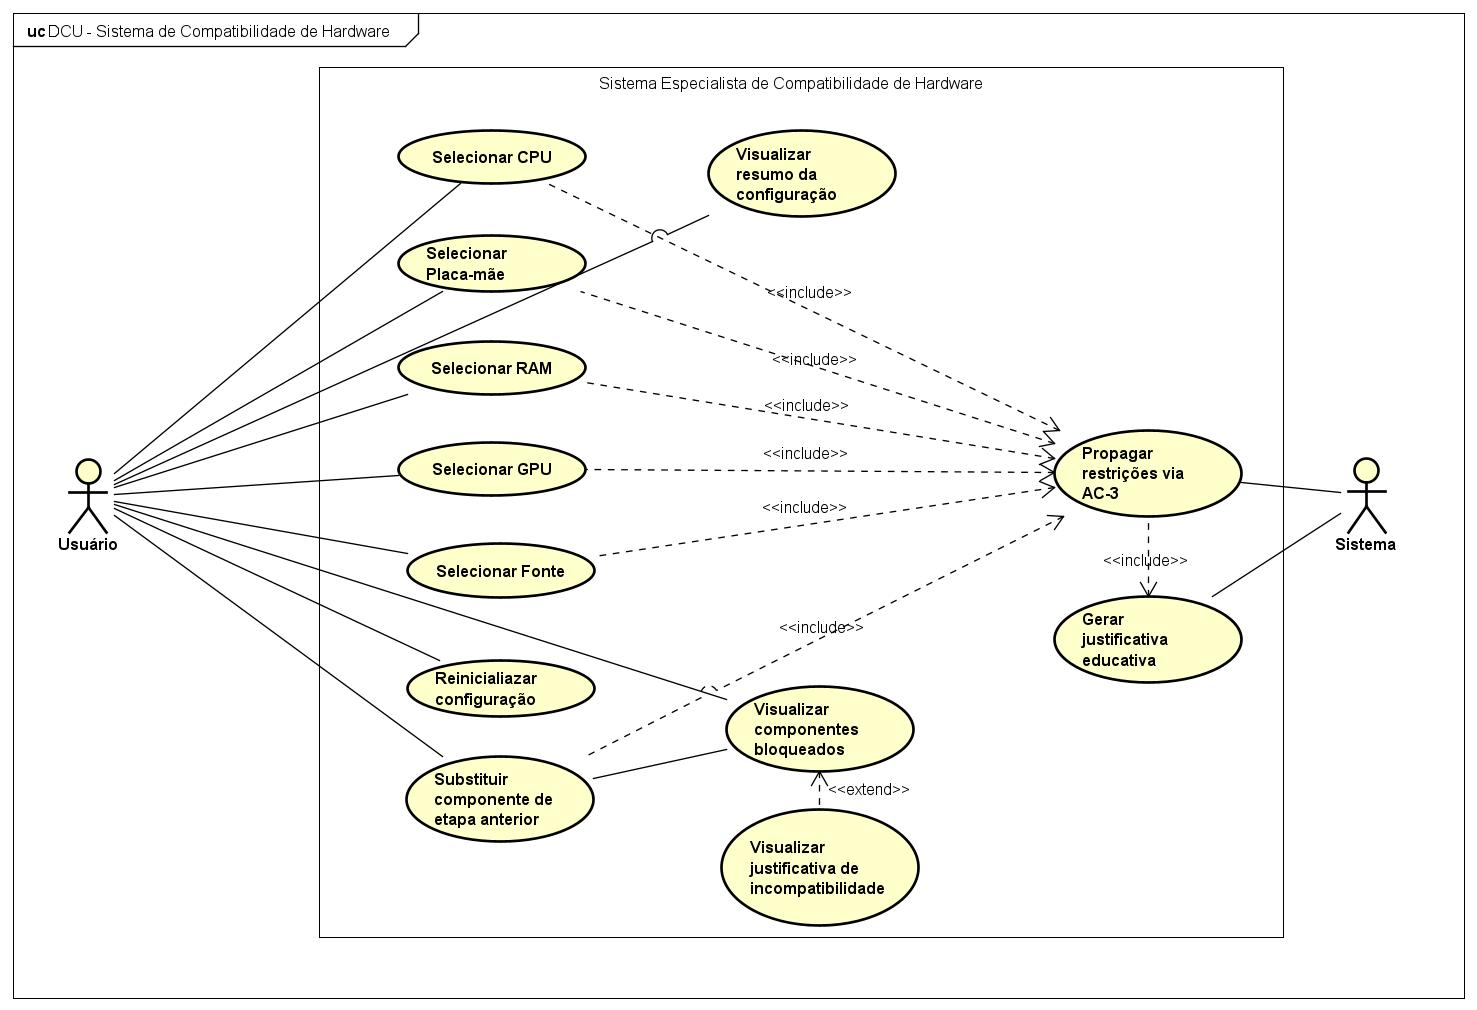
\includegraphics[width=1\textwidth]{imagens/DCU - Sistema de Compatibilidade de Hardware.jpg}
  \\\textbf{Fonte:} Elaborada pelo autor
  \label{fig:diagCasosDeUso}
\end{figure}
\FloatBarrier

\subsection{Especificação dos Casos de Uso}

Uma especificação de caso de uso fornece detalhe textual para um caso de uso.
A Tabela~\ref{tab:especCasosDeUso} apresenta o modelo de estrutura de tópicos
adotado para a especificação dos casos de uso deste trabalho (extraído de
\href{https://www.ibm.com/docs/pt-br/elm/6.0?topic=cases-use-case-specification-outline}{IBM-Especificação de Casos de Uso}).

\FloatBarrier
\begin{table}[!htbp]
  \centering
  \caption{Modelo para Especificação de Casos de Uso}
  \begin{tabular}{ c | p{11.5cm} }
    \hline
    \textbf{Item}        & \textbf{Descrição}                                                                                                                                                                                                                                                                                                                                                                                                                                                                                            \\ \hline
    Nome do Caso de Uso  &
    Declara o nome do caso de uso. Geralmente, o nome expressa o objetivo ou resultado observável do caso de uso, como ``Sacar Dinheiro'' no caso de um caixa eletrônico.                                                                                                                                                                                                                                                                                                                                                                \\ \hline
    Descrição Resumida   & Descreve a função e o objetivo do caso de uso.                                                                                                                                                                                                                                                                                                                                                                                                                                                                \\ \hline
    Fluxo de Eventos     & Apresenta o fluxo básico e os fluxos alternativos. O fluxo de eventos descreve o comportamento do sistema; ele não descreve como o sistema funciona, os detalhes da apresentação ou os detalhes da interface com o usuário. Se forem trocadas informações, o caso de uso deverá ser específico sobre o que será transmitido de um lado para outro. Por exemplo, em vez de descrever uma ação como ``o agente insere informações do cliente'', indique que ``o agente insere o nome e o endereço do cliente''. \\ \hline
    Fluxo Básico         & Descreve o comportamento principal ideal do sistema.                                                                                                                                                                                                                                                                                                                                                                                                                                                          \\ \hline
    Fluxos Alternativos  & Descreve exceções ou desvios do fluxo básico, como o comportamento do sistema quando o agente insere um ID de usuário incorreto e a autenticação do usuário falha.                                                                                                                                                                                                                                                                                                                                            \\ \hline
    Requisitos Especiais & Requisitos não-funcionais que são específicos para um caso de uso mas que não são especificados no texto do fluxo do caso de uso de eventos. Exemplos de requisitos especiais incluem estes fatores: requisitos legais e regulamentares; padrões de aplicativo; atributos de qualidade do sistema, incluindo usabilidade, confiabilidade, desempenho e capacidade de suporte; sistemas operacionais e ambientes; requisitos de compatibilidade e restrições de design.                                        \\ \hline
    Condições Prévias    & Um estado do sistema que deve estar presente antes de um caso de uso ser iniciado.                                                                                                                                                                                                                                                                                                                                                                                                                            \\ \hline
    Pós-Condições        & Uma lista de estados possíveis para o sistema imediatamente após a conclusão de um caso de uso.                                                                                                                                                                                                                                                                                                                                                                                                               \\ \hline
    Pontos de Extensão   & Um ponto no fluxo de eventos do caso de uso em que outro caso de uso é referenciado.                                                                                                                                                                                                                                                                                                                                                                                                                          \\ \hline
  \end{tabular}
  \\ \vspace{0.2cm}
  \textbf{Fonte:} Extraído de \href{https://www.ibm.com/docs/pt-br/elm/6.0?topic=cases-use-case-specification-outline}{IBM-Especificação de Casos de Uso}
  \label{tab:especCasosDeUso}
\end{table}
\FloatBarrier

A título de exemplo, a Tabela~\ref{tab:ucSelecionarComponente} apresenta a
especificação do caso de uso \textit{Selecionar Componente}, central ao fluxo de
configuração do sistema.

\FloatBarrier
\begin{table}[!htbp]
  \centering
  \caption{Especificação do Caso de Uso ``Selecionar Componente''}
  \begin{tabular}{ | p{15cm} | }
    \hline
    \textbf{Caso de Uso}                                                                                                                                                                                                                   \\
    Selecionar Componente                                                                                                                                                                                                                  \\	\hline
    \textbf{Referências}                                                                                                                                                                                                                   \\
    RF-01, RF-05, RF-09, RF-10                                                                                                                                                                                                             \\	\hline
    \textbf{Descrição Geral}                                                                                                                                                                                                               \\
    O caso de uso inicia-se quando o usuário seleciona um componente em uma das etapas do \textit{wizard} de configuração. O sistema dispara a propagação de restrições e atualiza a disponibilidade dos componentes nas etapas seguintes. \\	\hline
    \textbf{Atores}                                                                                                                                                                                                                        \\
    Usuário, Sistema                                                                                                                                                                                                                       \\	\hline
    \textbf{Pré-Condições}                                                                                                                                                                                                                 \\
    A base de conhecimento deve estar populada; o usuário deve estar em uma etapa válida do \textit{wizard}.                                                                                                                               \\	\hline
    \textbf{Garantia de Sucesso (Pós-Condições)}                                                                                                                                                                                           \\
    Componente registrado na configuração; domínios das categorias seguintes atualizados; componentes incompatíveis sinalizados com a respectiva justificativa.                                                                            \\	\hline
    \textbf{Requisitos Especiais}                                                                                                                                                                                                          \\
    A propagação deve ocorrer em tempo real (RNF-01); nenhum bloqueio pode ocorrer sem justificativa (RNF-14).                                                                                                                             \\	\hline
    \textbf{Fluxo Básico}
    \begin{enumerate}
      \item Usuário visualiza a lista de componentes da categoria atual;
      \item Usuário seleciona um componente compatível;
      \item Sistema registra a seleção e envia o estado completo à API REST;
      \item Sistema executa o algoritmo AC-3 sobre o grafo de restrições;
      \item Sistema poda os domínios das categorias seguintes e retorna os componentes disponíveis;
      \item Sistema apresenta a etapa seguinte com os componentes atualizados.
    \end{enumerate}
    \\	\hline
    \textbf{Fluxo Alternativo}
    \renewcommand{\labelenumii}{\arabic{enumi}.\arabic{enumii}}
    \begin{enumerate}
      \item Usuário tenta selecionar um componente incompatível
            \begin{enumerate}
              \item Sistema bloqueia a seleção e exibe a justificativa técnica da incompatibilidade (RF-10);
              \item Retorna ao passo 1.
            \end{enumerate}
    \end{enumerate}
    \\	\hline
  \end{tabular}
  \label{tab:ucSelecionarComponente}
\end{table}
\FloatBarrier

\section{Modelo de Domínio}

O modelo de domínio é um artefato de análise que representa os conceitos
relevantes do domínio do problema e os relacionamentos entre eles, sem
preocupação com detalhes de implementação \cite{larman2004}. Por se concentrar
no vocabulário do domínio, o modelo é elaborado apenas com as classes e seus
atributos, auxiliando na compreensão da aplicação. A
Figura~\ref{fig:modeloDeDominio} apresenta o modelo de domínio desenvolvido
neste trabalho.

O modelo reflete a decisão arquitetural de tornar a tripla $\langle X, D, C
  \rangle$ do CSP configurável. Em vez de especializar a classe \textit{Componente}
em subclasses fixas (CPU, Placa-mãe, RAM, GPU e Fonte), com atributos codificados,
adota-se uma estrutura genérica baseada em metadados: a classe \textit{Categoria}
representa as variáveis ($X$); a classe \textit{Componente} representa os valores
de domínio ($D$); a classe \textit{Caracteristica} define, por categoria, os
atributos configuráveis, cujos valores são registrados em
\textit{ComponenteCaracteristica}; e a classe \textit{Restricao} representa o
conjunto $C$, associando duas características por meio de um operador. Essa
organização realiza concretamente os requisitos RNF-07 e RNF-08, uma vez que a
inclusão de novas categorias, características ou restrições não exige alteração de
código, apenas a inserção de novos registros na base de conhecimento.

\FloatBarrier
\begin{figure}[!htbp]
  \centering
  \caption{Modelo de Domínio}
  %scale redimensiona a figura.
  %1.5 = 150% do tamanho original
  %1 = 100% do tamanho original
  %0.20 = 20% do tamanho original
  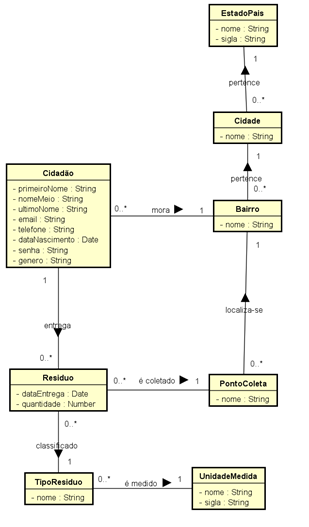
\includegraphics[width=1\textwidth]{imagens/ModelodeDominio.png}
  \\\textbf{Fonte:} Elaborada pelo autor
  \label{fig:modeloDeDominio}
\end{figure}
\FloatBarrier

% \section{Diagrama de Objetos}
% Fazer uma pequena definição de diagrama de objetos para introduzir essa seção. Terminar o parágrafo informando qual figura apresenta o diagrama de objetos. Elabore o diagrama de objetos para cada classe identificada no modelo de domínio.


\section{Diagrama de Classes de Análise}

O diagrama de classes de análise é uma evolução do modelo de domínio que
incorpora, além dos atributos, os métodos que descrevem o comportamento das
classes, aproximando o modelo da estrutura que será implementada
\cite{larman2004}. A Figura~\ref{fig:classesDeAnalise} apresenta o diagrama de
classes de análise elaborado neste trabalho.

Em relação ao modelo de domínio, o diagrama acrescenta os métodos responsáveis
pela lógica do sistema. A classe \textit{Restricao} recebe o método
\textit{isSatisfeita}, que avalia se os valores de duas características atendem ao
operador definido; a classe \textit{ComponenteCaracteristica} expõe o método de
acesso ao valor; e são introduzidas as classes de saída do motor de inferência,
\textit{ResultadoValidacao} e \textit{JustificativaEducativa}, responsáveis por
transportar, respectivamente, o resultado da propagação e as justificativas
educativas exibidas ao usuário. Diferentemente das classes da base de
conhecimento, essas duas classes não são persistidas, sendo geradas a cada
execução do AC-3.

\FloatBarrier
\begin{figure}[!htbp]
  \centering
  \caption{Diagrama de Classes de Análise}
  %scale redimensiona a figura.
  %1.5 = 150% do tamanho original
  %1 = 100% do tamanho original
  %0.20 = 20% do tamanho original
  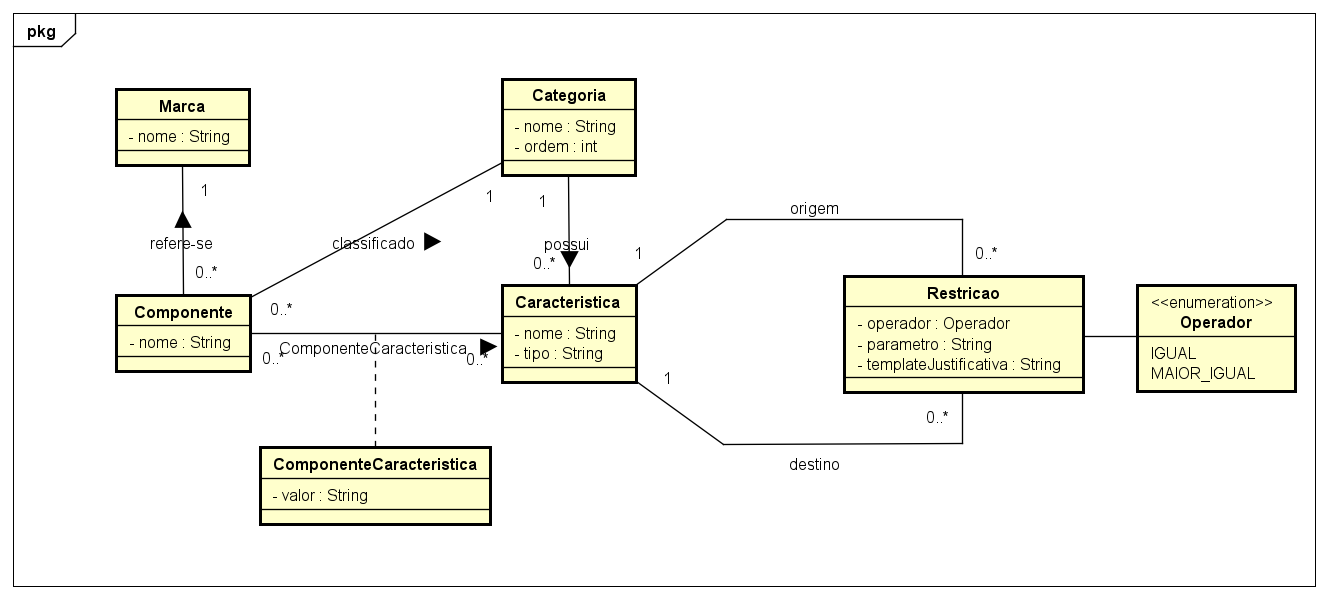
\includegraphics[width=1\textwidth]{imagens/diagrama-classe-v2.png}
  \\\textbf{Fonte:} Elaborada pelo autor
  \label{fig:classesDeAnalise}
\end{figure}
\FloatBarrier

\section{Diagrama de Atividades}

Um diagrama de atividades ilustra a natureza dinâmica de um sistema pela
modelagem do fluxo de controle de uma atividade à outra. Uma atividade
representa uma operação em alguma classe do sistema que resulta em uma mudança de
estado. Tipicamente, diagramas de atividades são usados para modelar fluxos de
processos, processos de negócios ou operações internas. Embora seja semelhante a
uma máquina de estados, o diagrama de atividades tem propósito distinto, voltado
a capturar ações e seus resultados em termos de mudanças no estado do objeto.

O fluxo é mostrado por meio de transições, representadas por setas direcionadas
que indicam o caminho entre os estados de atividade (ação). Um diagrama de
atividades é normalmente composto pelos seguintes elementos: atividades (ações),
estados de atividade (ação), transição, fluxo de objeto, estado inicial, estado
final, \textit{branching}, sincronização e raias.

% \FloatBarrier
% \begin{figure}[!htbp]
%   \centering
%   \caption{Diagrama de Atividades}
%   \includegraphics[width=1\textwidth]{imagens/Diagrama de Atividades.png}
%   \\\textbf{Fonte:} Elaborada pelo autor
%   \label{fig:diagramaDeAtividades}
% \end{figure}
% \FloatBarrier